% ----------------------------------------------------------------
% Customization by Leandro C. Coelho -----------------------------
% ----------------------------------------------------------------
\documentclass[12pt, twoside]{report}

\newcommand{\citeny}[1]{\citename{#1}~\citeyear{#1}}

% Setup TikZ
\usepackage{tikz}
\usetikzlibrary{arrows}
\tikzstyle{block}=[draw opacity=0.7,line width=1cm]

\usepackage{graphicx}
\usepackage[lofdepth,lotdepth]{subfig}
\usepackage{amsmath, amsthm, amsfonts}
\usepackage[numbers]{natbib}
\usepackage{algorithm, algorithmic}
\usepackage{placeins}
\usepackage{rotating}
\usepackage{booktabs}
\usepackage{multirow}
\usepackage{physics,empheq} 
\usepackage[font=small,labelfont=bf,tableposition=top]{caption}
\usepackage{xfrac}
\usepackage{relsize}
\usepackage{mathrsfs}
%\setcounter{secnumdepth}{5}
\usepackage{lineno}

\usepackage[text={16cm,23cm},centering]{geometry}

\setlength{\parskip}{1.2ex}
\setlength{\parindent}{0em}
\clubpenalty = 100
\widowpenalty = 100
\renewcommand{\baselinestretch}{1.5}

\newcommand*{\red}{\textcolor{red}}
\newcommand*{\green}{\textcolor{green}}
\newcommand*{\blue}{\textcolor{blue}}
\everymath{\displaystyle}
\begin{document}

\setpagewiselinenumbers

%\modulolinenumbers[5]
%\linenumbers

\title{Quantum Nano engines (fix title)}

\date{2019}



\author{Archisman Panigrahi\\
	\footnotesize Indian Institute of Science, Bangalore\\
	\footnotesize \texttt{\{archismanp@iisc.ac.in\}} \\ }


\maketitle

\begin{abstract}

Make abstruct
Todo. 1. sinusodially spelling
2. add graphs for coherent and squeezed state.

\end{abstract}
%{\bf Keywords:} enter, keyword, here.

\tableofcontents

\section{Introduction}
The classical limits of the maximum achievable efficiency of an ideal heat engine running between temperatures $T_{hot}$ and $T_{cold}$ us given by Carnot's formula $\eta_{Carnot} = 1 - \frac{T_{cold}}{T_{hot}}$.\\
The efficiency of real engines are, however, a fraction of this ideal formula, as the reversible Carnot engine is inifinitely slow, and there are frictional dissipations in the real world.
Nano engines based on the principles of Quantum Mechanics can achieve much higher efficiencies than their classical counterparts and can have efficiency close to the Carnot limit.
These engines have been realized in many forms including of ion traps[ref], three level systems[ref],harmonic oscillators [ref].
It has been shown both theoretically[Abah] and experimentally[Klaers] that the efficiencies of engines realized using ``squeezed harmonic oscillators" an even surpass the Carnot limit, without violating the second law of thermodynamics. In this report, it will be elaborated in which sense the Carnot limit is surpassed, and why the second law is not violated.
To see how the experiment[ref Klaers] was done, let us recap squeezed states of harmonic oscillator and Brownian motion.
\section{Theory of the for Brownian Harmonic oscillator}

Before we discuss squeezed states, let us review ``Coherent states" of a harmonic oscillator.
\subsection{Coherent states}
The position and momentum of classical harmonic oscillator (a particle of mass $m$ in potential $\frac{1}{2}m\omega^2x^2$)  oscillates with period $\omega$, its natural frequency.
However, in quantum mechanics, the expectation value of position or momentum of an eigenstate of the Hamiltonian does not change with time.


For the harmonic oscillator, the Hamiltonian is $\hat{H} = \frac{\hat{p}^2}{2m} + \frac{1}{2}m \omega^2 {\hat{x}}^2$.


Let the eigenstates of $\hat{H}$ be denoted by $\ket{n}$. It can be shown (ref. Cohen Tannoudji) that it has energy $E_n = (n+\frac{1}{2}) \hbar\omega$. The state evolves with time as $\ket{n,t} = e ^ { -i \left( n + \frac { 1 } { 2 } \right) \omega t } \ket{n,t=0}$, and will have equal energies $(n+\frac{1}{2}) \frac{\hbar\omega}{2}$ in position and momentum coordinates. And, the expected values of position and momentum are $0$ and do not change over time.
There exist quantum states whose expected values of position and momentum oscillate sinusoidally with time, and the wave packet does not spread with time. These are known as ``Coherent states".


Let us define $x_0 = \sqrt{\frac{\hbar}{m\omega}}$ and $p_0 = \sqrt{\hbar m \omega}$, and dimensionless operators $\hat{X} = \frac{\hat{x}}{x_0}$,$\hat{P} = \frac{\hat{p}}{p_0}$. Then we can rewrite $\hat{H} = \frac{\hbar\omega}{2}({\hat{X}}^2 + {\hat{P}}^2)$. Let us define two non Hermitian operators $\hat{a} = \frac{\hat{X} + i \hat{P}}{\sqrt{2}}$, and ${\hat{a}}^\dagger = \frac{\hat{X} - i \hat{P}}{\sqrt{2}}$. Then, $[\hat{a},\hat{a}^\dagger] = 1$, and the Hamiltonian can be written as $\hat{H} = \hbar\omega( \hat{a}^\dagger \hat{a} + \frac{1}{2})$.
$\hat{a}^\dagger$ and $\hat{a}$ are known as ``creation" and ``annihilation" operators, respectively, because they act on the eigenstates as follows. 
\begin{equation}\label{eq:a} { \hat{a} | n \rangle = \sqrt { n } | n - 1 \rangle } \end{equation}
\begin{equation} \label{eq:adagger}{ \hat{a} ^ { \dagger } | n \rangle = \sqrt { n + 1 } | n + 1 \rangle }\end{equation} 
We can define $\hat{N} = \hat{a}^\dagger\hat{a}$, and then, $\hat{N} \ket{n} = n\ket{n}$, denoting the number of excitations (e.g. photons or phonons) in the system. The creation and annihilation operators can be viewed as operators which create or destroy such an excitation, respectively, hence their name.

The operator $\hat{a}$ acts on $\ket{0}$ (the vaccuum state) to give the zero vector of the Hilbert space. However, there exist states which are eigenstates of the annihilation operator, and these states are known as the coherent states. (ref. Wikipedia)

Let \begin{equation}\label{eq:coherent}
	\hat {a} | \alpha \rangle = \alpha | \alpha \rangle
\end{equation}, where $\alpha$ is a complex number, and $\ket{\alpha}$ is a coherent state. Since $\ket{n}$ form a basis of the Hilbert space, $\exists c_n \in \mathbb{C}$, such that \begin{equation} \label{eq:coherentexpansion}| \alpha \rangle = \displaystyle\sum _ { n = 0 } ^ { \infty } c_n | n \rangle \end{equation}
$\begin{aligned}\text{From equations (\ref{eq:coherent}) and (\ref{eq:coherentexpansion}), we get,}\displaystyle\sum _ { n = 0 } ^ { \infty } c_ { n } \hat {a} | n \rangle &= \sum _ { n = 0 } ^ { \infty } \alpha c_{ n } | n \rangle\\\implies \sum _ { n = 1 } ^ { \infty } c_{ n } \sqrt { n } | n - 1 \rangle &= \sum _ { n = 0 } ^ { \infty } \alpha c_{ n } | n \rangle \\ \implies \sum _ { n = 0 } ^ { \infty } c _ { n + 1 } \sqrt { n + 1 } | n \rangle &= \sum _ { n = 0 } ^ { \infty } \alpha c _ { n } | n \rangle\\ \implies \quad c _ { n + 1 } \sqrt { n + 1 } &= \alpha c _ { n } \\  \implies \frac { c _ { n + 1 } \sqrt { ( n + 1 ) ! } } { \alpha ^ { n + 1 } }  &= \frac { c _ { n } \sqrt { n ! } } { \alpha ^ { n } } \\  &= \frac { c _ { 0 } \sqrt { 0 ! } } { \alpha ^ { 0 } }  \\ \implies c _ { n } &= c _ { 0 } \frac { \alpha ^ { n } } { \sqrt { n ! } }\end{aligned}$\\
Since $\displaystyle\sum _ { n = 0 } ^ { \infty } \left| c _ { n } \right| ^ { 2 } = 1 \implies c _ { 0 } = e ^ { - \frac { | \alpha | ^ { 2 } } { 2 } }$. Finally we get $\displaystyle| \alpha \rangle = e ^ { - \frac {|\alpha| ^ { 2 } } { 2 } } \sum _ { n = 0 } ^ { \infty } \frac { \alpha ^ { n } } { \sqrt { n ! } } | n \rangle$,
and $\displaystyle| \alpha,t \rangle = e ^ { - \frac {|\alpha| ^ { 2 } + i\omega t} { 2 }} \sum _ { n = 0 } ^ { \infty } \frac { (\alpha e^{-i\omega t})^ { n }  } { \sqrt { n ! } } | n \rangle$. So the state remains a coherent state over time, only the parameter $\alpha$ evolves as $\alpha(t) = \alpha(0) e^{-i\omega t}$.
Now, 
\begin{equation}
\begin{cases}

	&{ \langle \hat{a} \rangle = \alpha }\\
	&{ \langle \hat{a}^\dagger \rangle = \alpha^* }\\
	&{ \langle x \rangle = x _ { 0 } \left( \frac { \hat{a}+ \hat{a} ^ { \dagger } } { 2 } \right) = x _ { 0 } \frac{\alpha + \alpha^*}{2}}\\
	& { \langle p \rangle = p_0  \left\langle \frac { \hat{a}- \hat{a} ^ { \dagger } } { \sqrt { 2 } i } \right\rangle =  p_0 \frac{\alpha - \alpha^*}{2i} }\\
	& { \langle \hat{x}^2 \rangle = {x_0}^2  \left\langle \frac { \hat{a}^2 + \hat{a^ { \dagger }}^2 + \hat{a}\hat{a}^\dagger + \hat{a}^\dagger \hat{a} } { 2 } \right\rangle =  \frac{\alpha^2 + \alpha^{*2} + 2|\alpha|^2 + 1 }{2}{x_0}^2}\\
	& { \langle \hat{p}^2 \rangle = {p_0}^2  \left\langle \frac { \hat{a}^2 + \hat{a^ { \dagger }}^2 - \hat{a}\hat{a}^\dagger - \hat{a}^\dagger \hat{a} } { -2 } \right\rangle = \frac{ 2|\alpha|^2 + 1 -\alpha^2 - \alpha^{*2} }{2}{p_0}^2}\\
	& \expval{E} = \frac{\hbar\omega}{2}(\hat{a}^{\dagger}\hat{a}+1) = \frac{\hbar\omega}{2}(|\alpha|^2 + 1)\\
	& (\Delta x)^2 = \frac{{x_0}^2}{2}\\
	& (\Delta p)^2 = \frac{{p_0}^2}{2}\\
	& \Delta x \cdot \Delta p = x_0 p_0 = \frac{\hbar}{2} 
	
	\end{cases}\end{equation}
Now let $\alpha = |\alpha|e^{i\phi}$. Then, $\langle x \rangle (t) $$= \sqrt{2} x_0 \Re{\alpha(t)} $$= \sqrt{2} x_0 |\alpha| \cos(\phi-\omega t)$, and $ \langle p \rangle (t) $$= \sqrt{2} p_0 \Im{\alpha(t)} $$= \sqrt{2} x_0 |\alpha| \sin(\phi-\omega t)$. The total energy ,the standard deviations in position and momentum remain constant, while the expected position and momentum vary sinusodially with time, just like a classical particle. Solving the first order differential equation obtained from (\ref{eq:coherent}) in position basis, it can be easily shown that the wave function $\psi_\alpha (x) = \braket{x}{\alpha}$ is a Gaussian, and its mean $\expval{x}$ changes sinusodially with time.

\begin{figure}
	\centering
	\subfloat[Subfigure 1 list of figures text][Subfigure 1 caption]{
		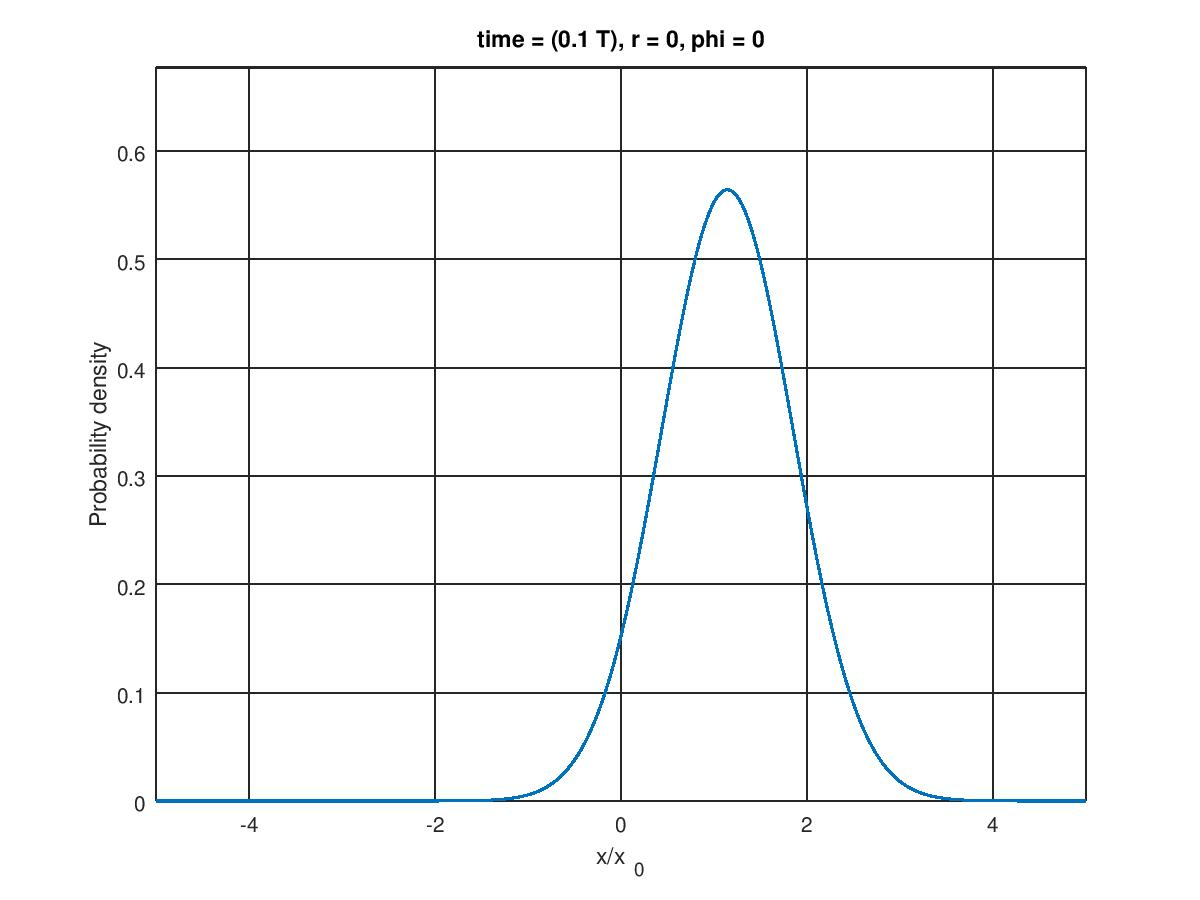
\includegraphics[width=0.4\textwidth]{graphs/coherent/1.jpg}
		\label{fig:subfig1}}
	\qquad
	\subfloat[Subfigure 2 list of figures text][Subfigure 2 caption]{
		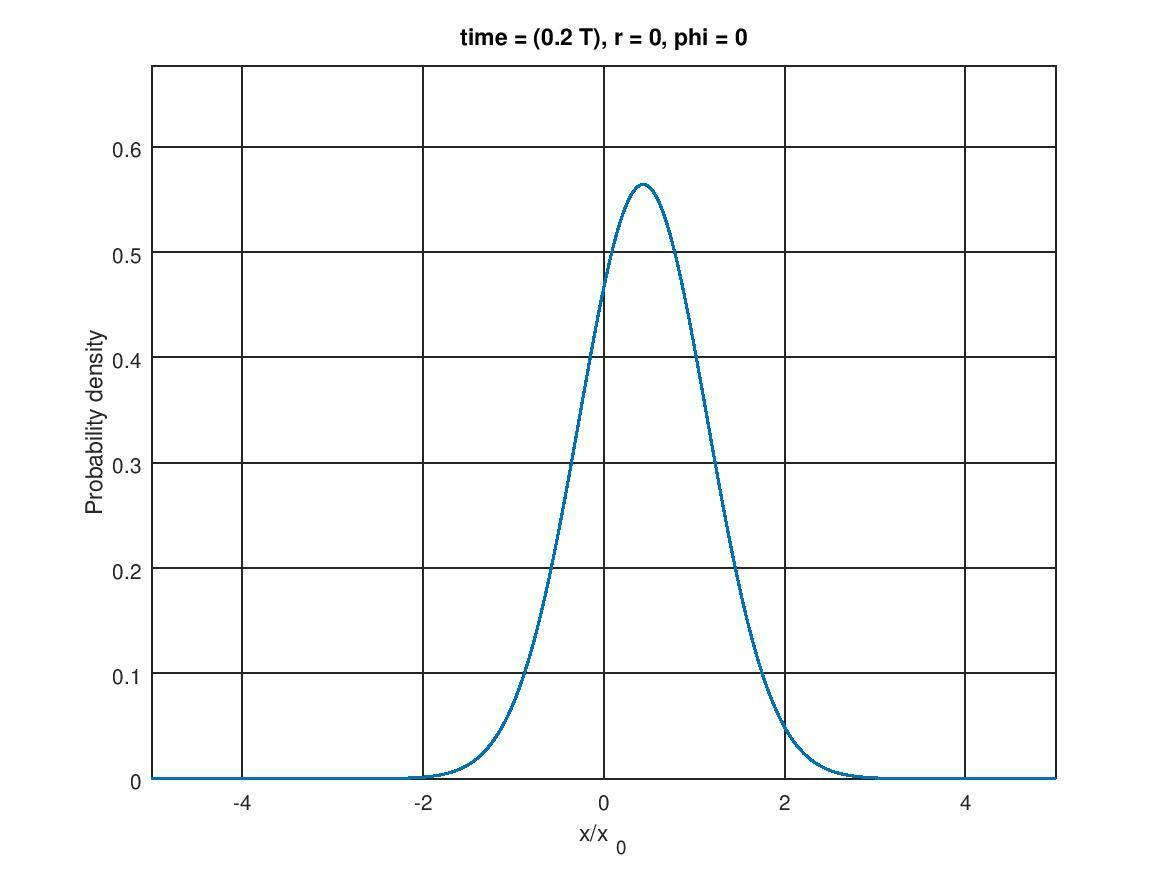
\includegraphics[width=0.4\textwidth]{graphs/coherent/2.jpg}
		\label{fig:subfig2}}
	\subfloat[Subfigure 3 list of figures text][Subfigure 3 caption]{
		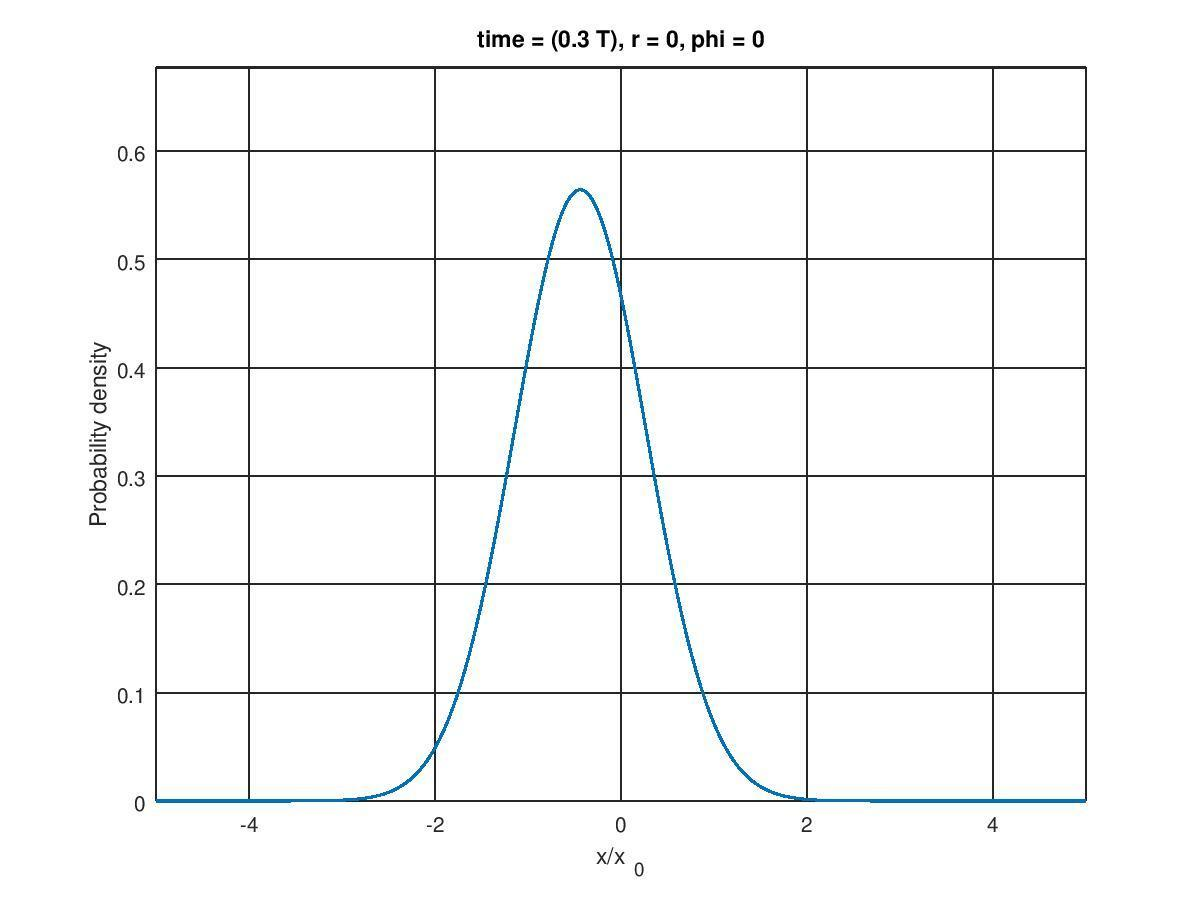
\includegraphics[width=0.4\textwidth]{graphs/coherent/3.jpg}
		\label{fig:subfig3}}
	\qquad
	\subfloat[Subfigure 4 list of figures text][Subfigure 4 caption]{
		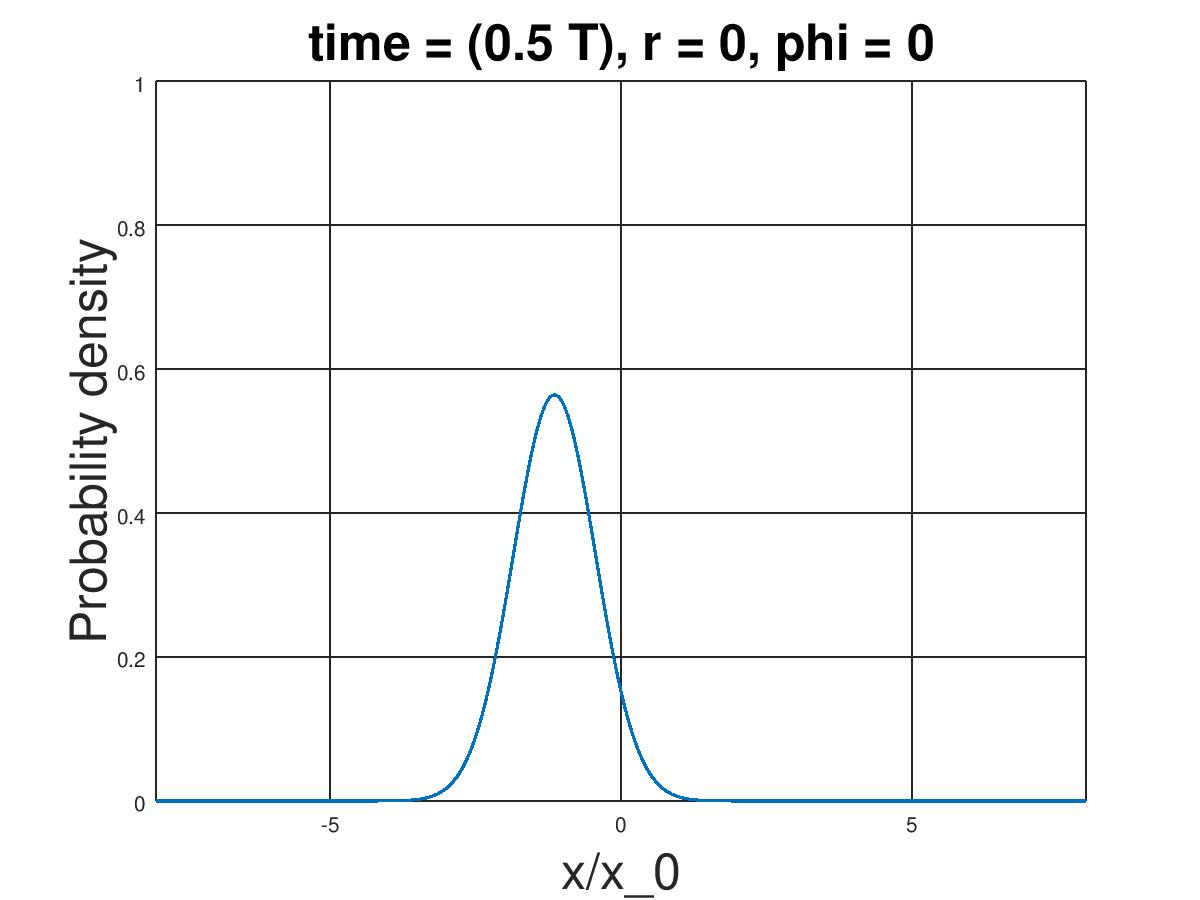
\includegraphics[width=0.4\textwidth]{graphs/coherent/4.jpg}
		\label{fig:subfig4}}
		\subfloat[Subfigure 2 list of figures text][Subfigure 2 caption]{
		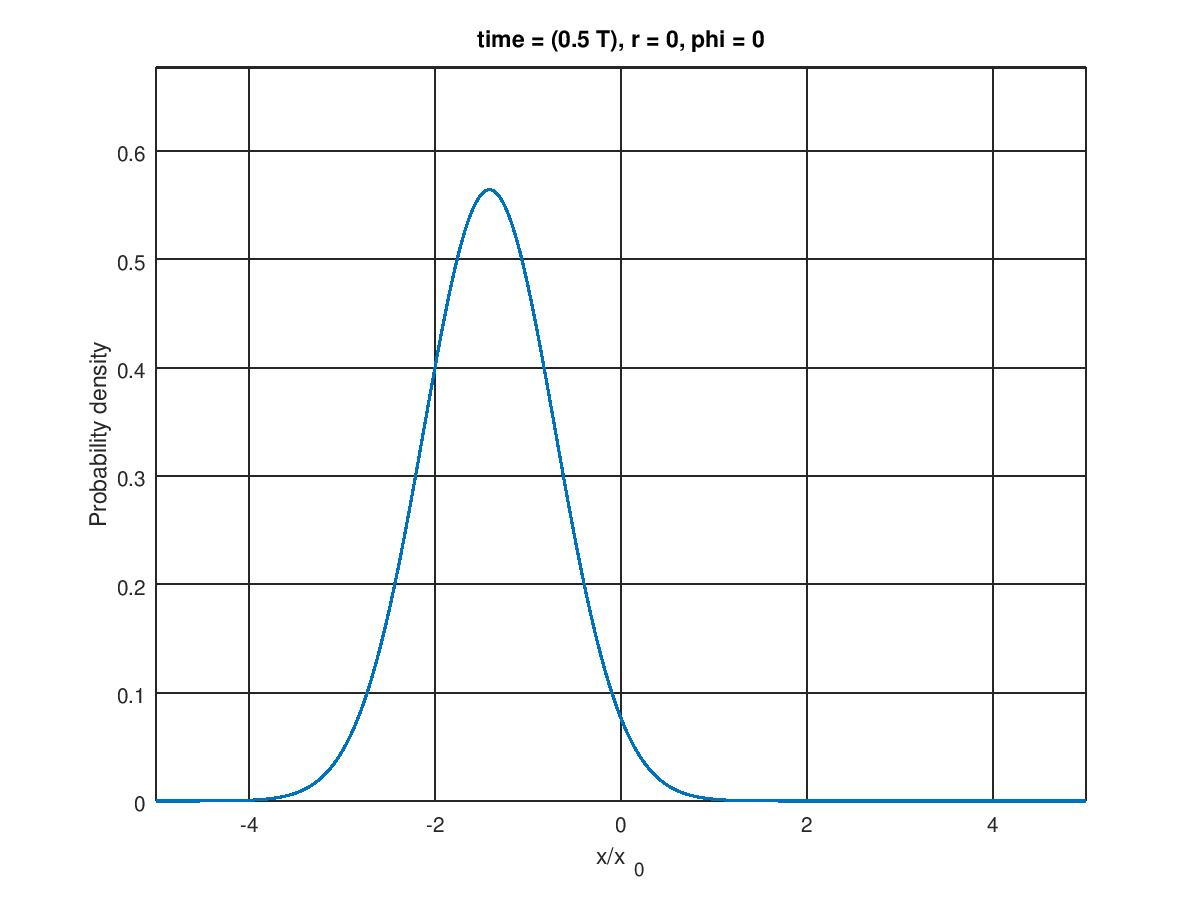
\includegraphics[width=0.4\textwidth]{graphs/coherent/5.jpg}
		\label{fig:subfig2}}
	\qquad
	\subfloat[Subfigure 3 list of figures text][Subfigure 3 caption]{
		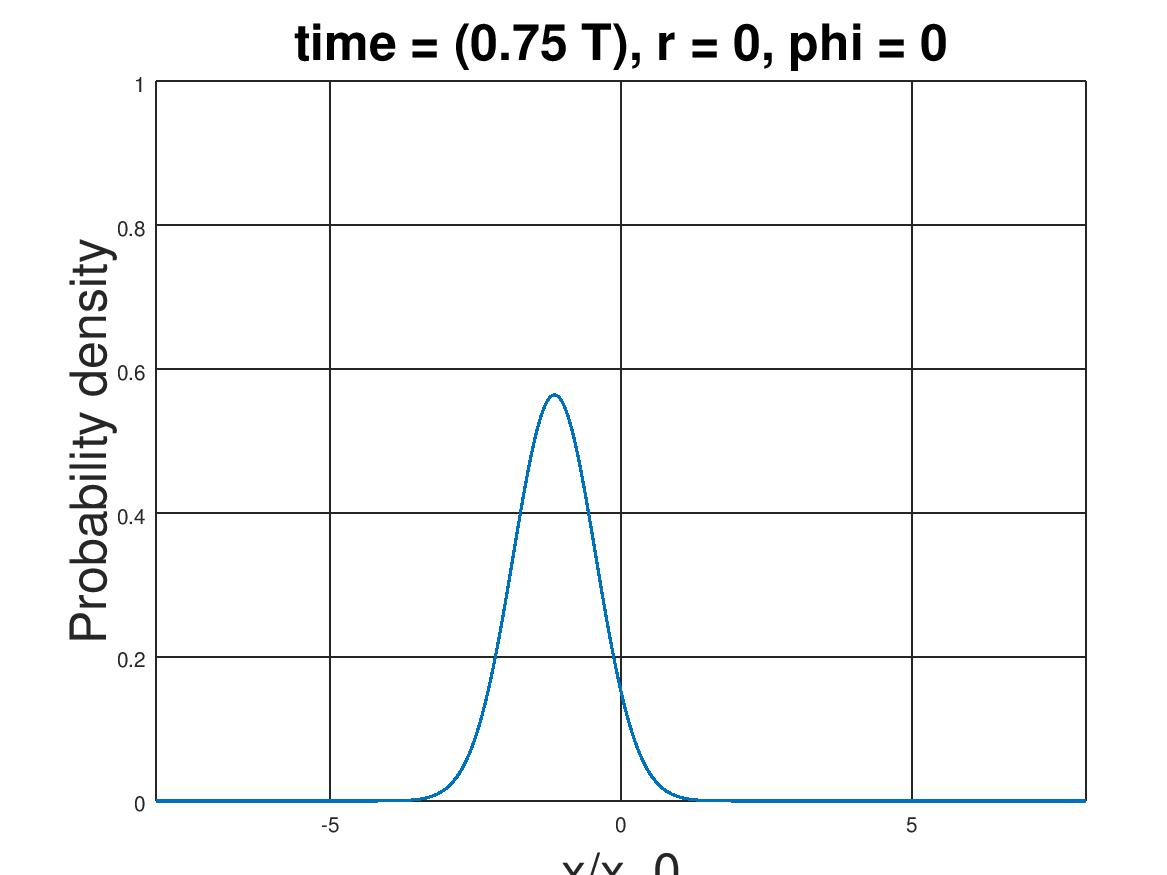
\includegraphics[width=0.4\textwidth]{graphs/coherent/6.jpg}
		\label{fig:subfig3}}
	\qquad
	\subfloat[Subfigure 3 list of figures text][Subfigure 3 caption]{
		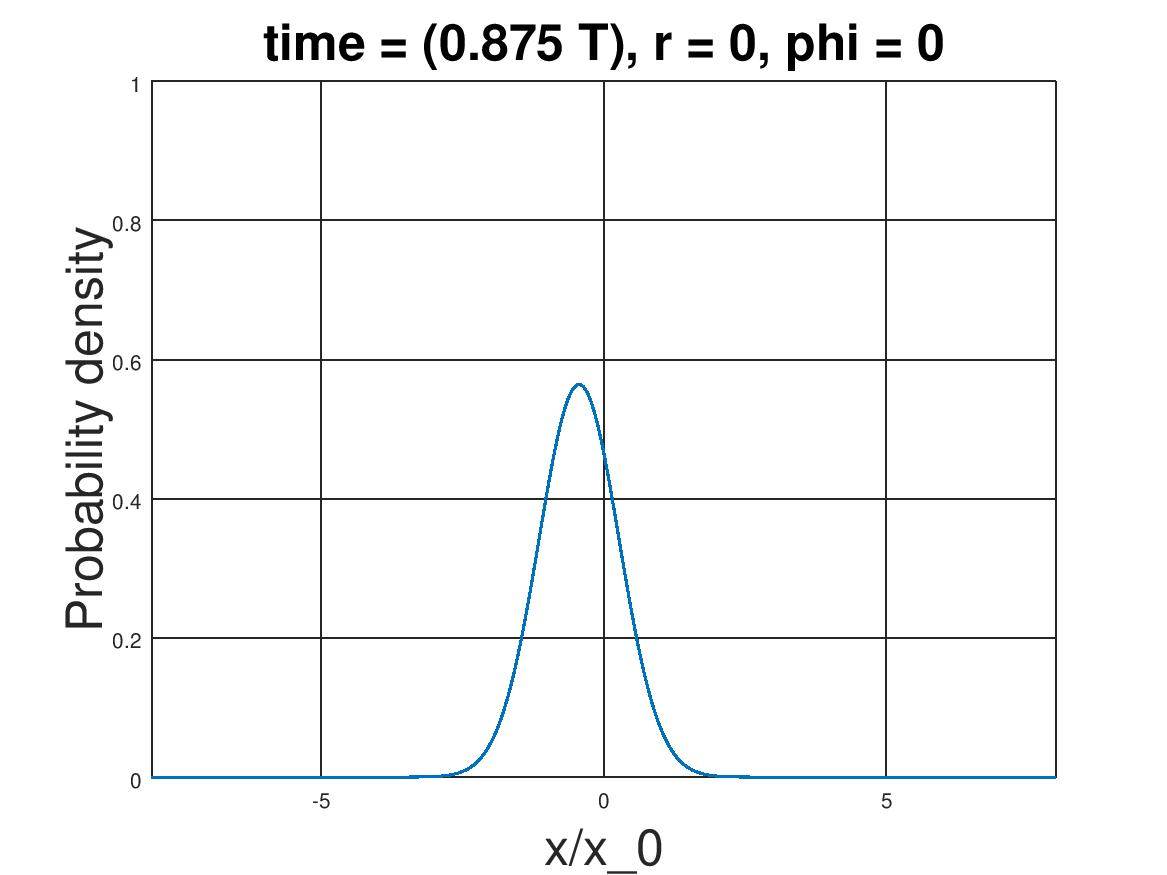
\includegraphics[width=0.4\textwidth]{graphs/coherent/7.jpg}
		\label{fig:subfig3}}
	\qquad
	\subfloat[Subfigure 3 list of figures text][Subfigure 3 caption]{
		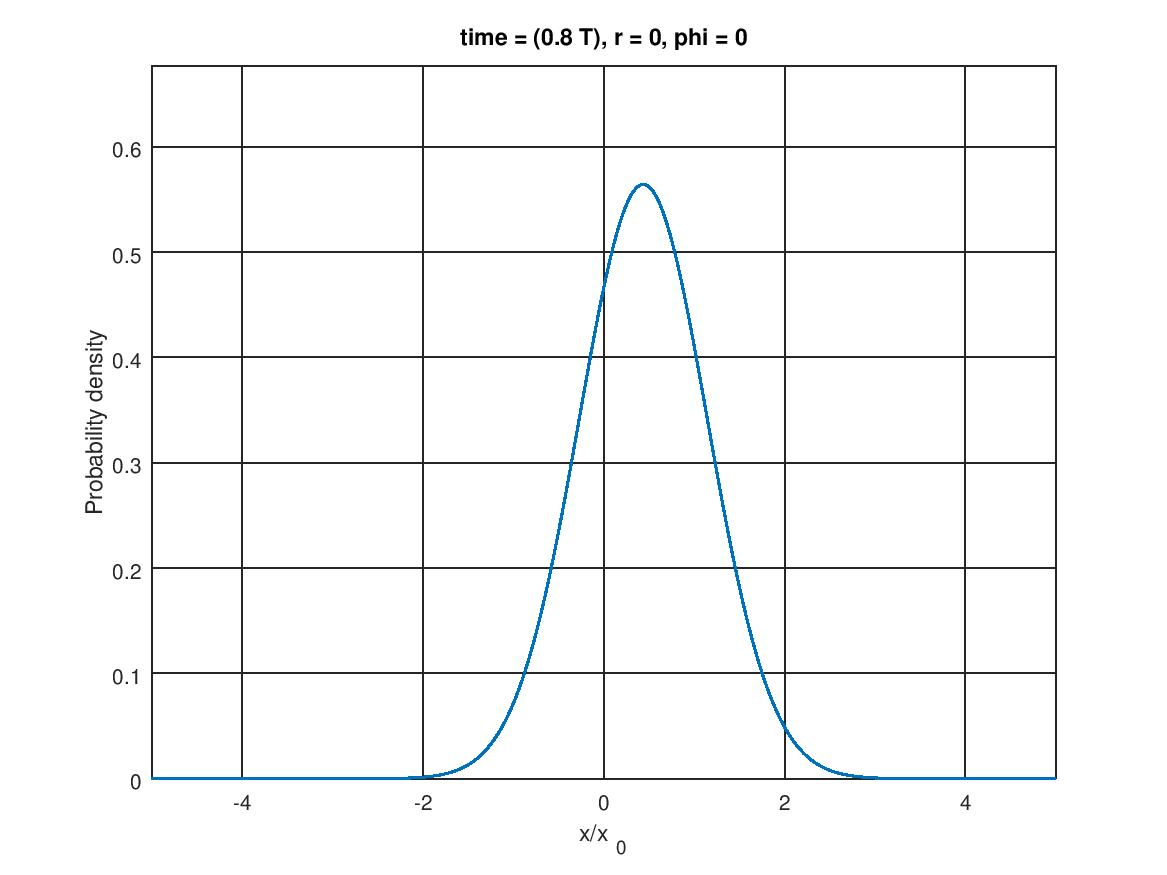
\includegraphics[width=0.4\textwidth]{graphs/coherent/8.jpg}
		\label{fig:subfig3}}
	\qquad
	\subfloat[Subfigure 3 list of figures text][Subfigure 3 caption]{
		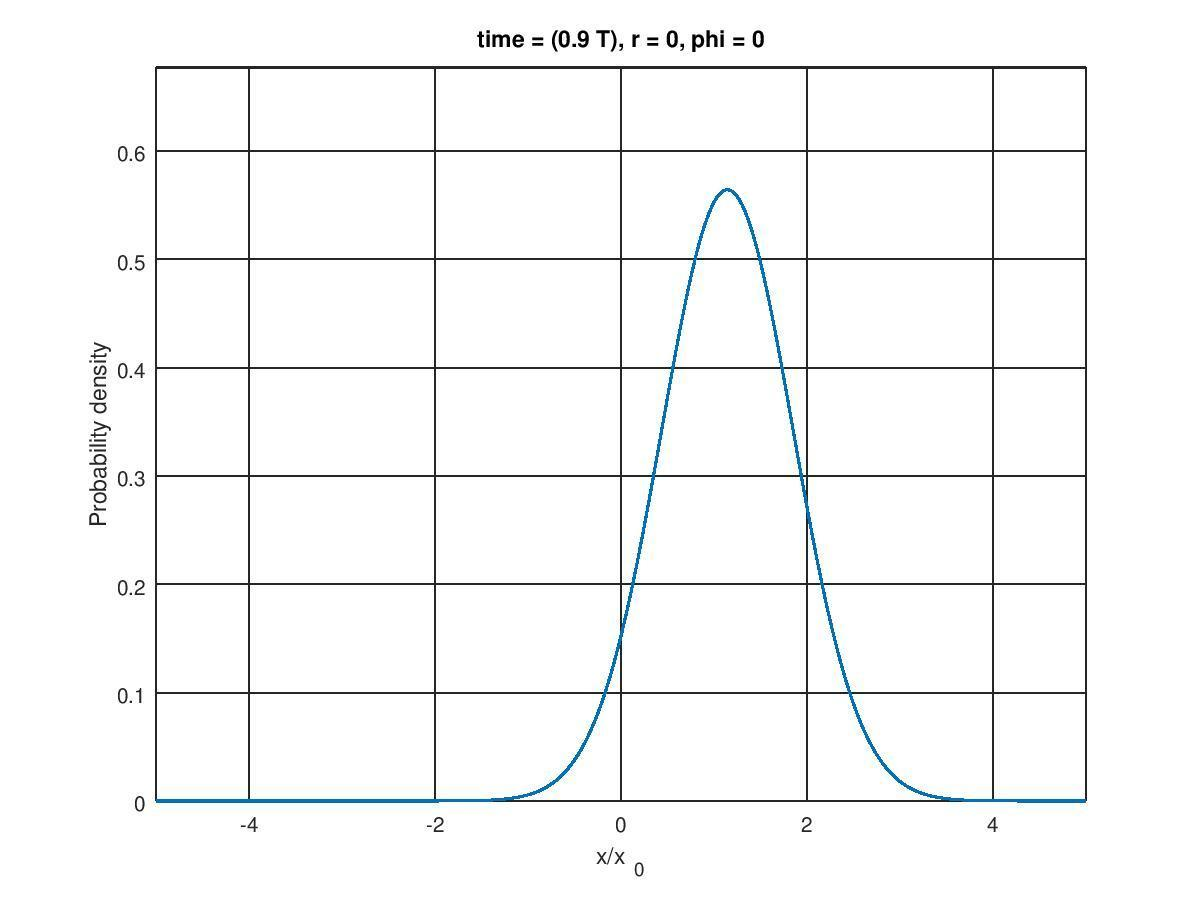
\includegraphics[width=0.4\textwidth]{graphs/coherent/9.jpg}
		\label{fig:subfig3}}
	\qquad
	\subfloat[Subfigure 3 list of figures text][Subfigure 3 caption]{
		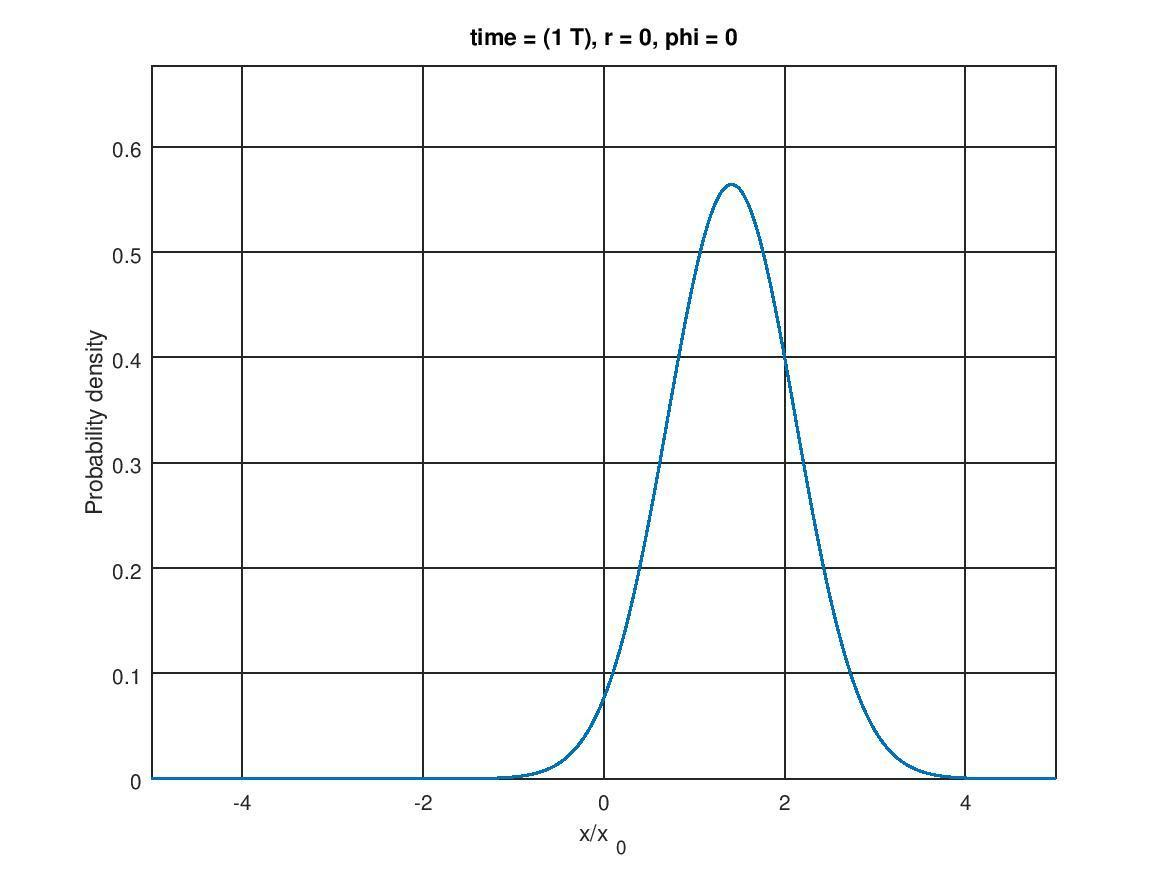
\includegraphics[width=0.4\textwidth]{graphs/coherent/10.jpg}
		\label{fig:subfig3}}
	\qquad
	\subfloat[Subfigure 3 list of figures text][Subfigure 3 caption]{
		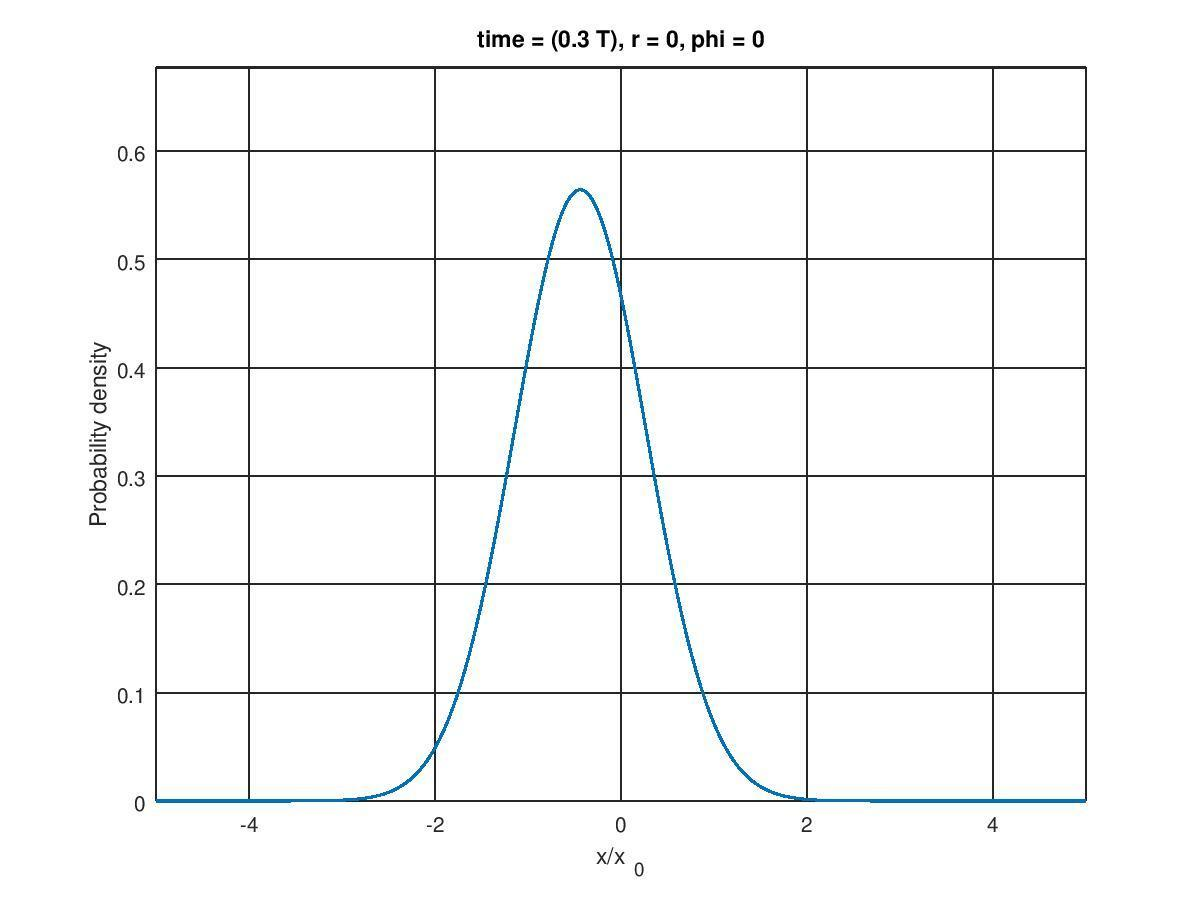
\includegraphics[width=0.4\textwidth]{graphs/coherent/3.jpg}
		\label{fig:subfig3}}
	\qquad
	\subfloat[Subfigure 3 list of figures text][Subfigure 3 caption]{
		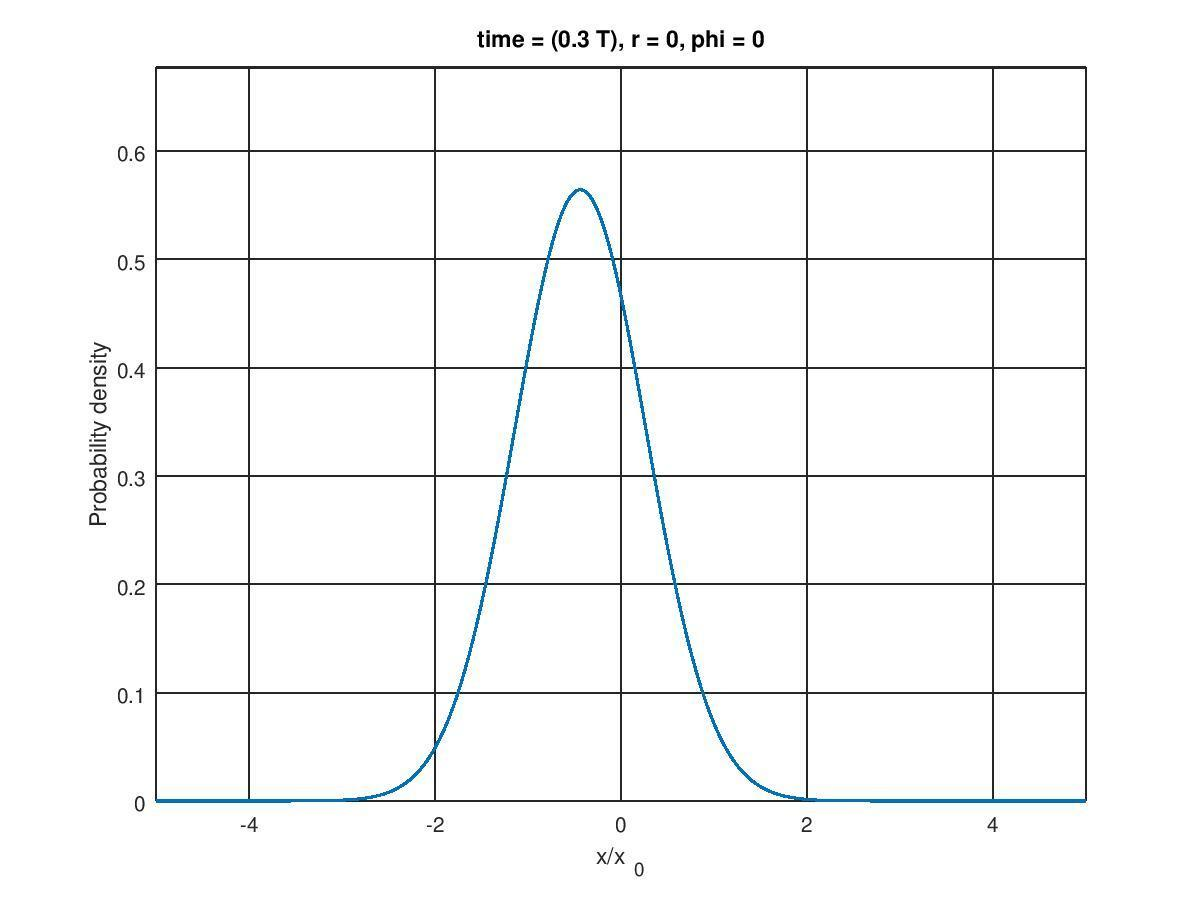
\includegraphics[width=0.4\textwidth]{graphs/coherent/3.jpg}
		\label{fig:subfig3}}
	\qquad
	\subfloat[Subfigure 3 list of figures text][Subfigure 3 caption]{
		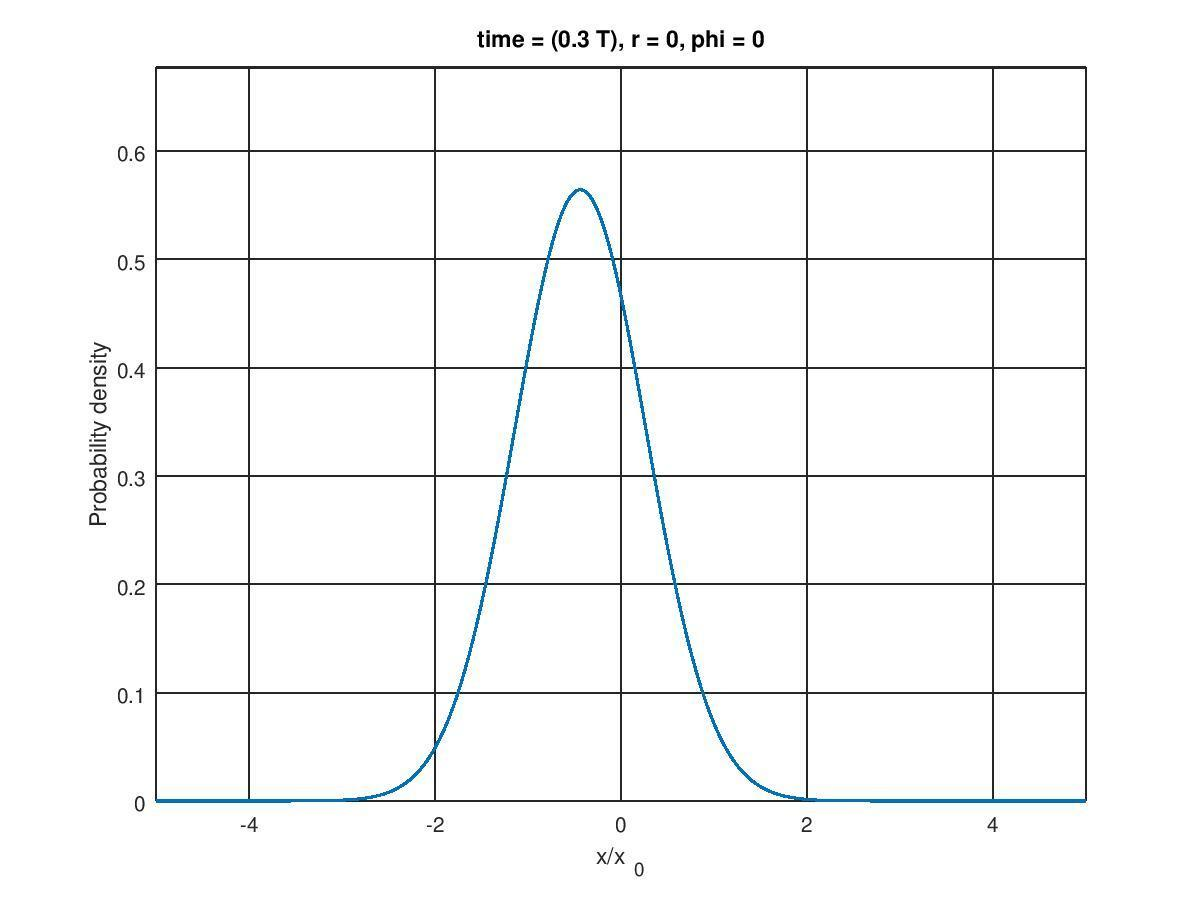
\includegraphics[width=0.4\textwidth]{graphs/coherent/3.jpg}
		\label{fig:subfig3}}
	\qquad
	\caption{This is a figure containing several subfigures.}
	\label{fig:globfig}
\end{figure}
	
	
\subsection{Squeezed states}

The coherent state behaves like a classical particle in a harmonic potential, and it has equal uncertainty in position and momentum. However, there exist states which have different values of standard deviation in position and momentum coordinates. In the next section, we will see that the uncertainty is related to the effective temperature in these coordinates, and this can be utilized to prepare efficient heat engines. Let us define \begin{equation} \label{eq:squeeze}
\hat{Q} = \lambda \hat{a} + \mu \hat{a}^\dagger
\end{equation} where $|\lambda|^2 - |\mu|^2 = 1$. Let $\lambda = \cosh(r)$, $\mu = \sinh(r)e^{i\phi}$, where $r,\phi \in \mathbb{R}$. The eigenstates of $\hat{Q}$ are defined as the squeezed states. (reference of squeezed state).
 We have,
 \[  \left( \begin{array} { l } { \hat { Q } } \\ { \hat { Q } ^ { \dagger } } \end{array} \right) = \left( \begin{array} { l l } { \lambda } & { \mu } \\ { \mu ^ { * } } & { \lambda ^ { * } } \end{array} \right) \left( \begin{array} { l } { \hat{a} } \\ { \hat{a}^\dagger } \end{array} \right)\]
 
 Inverting, we get, 
 \begin{equation}
\left( \begin{array} { l } { \hat { a } } \\ { \hat { a } ^ { \dagger } } \end{array} \right) = \left( \begin{array} { c c } { \lambda^* } & { - \mu } \\ { - \mu ^ { * } } & { \lambda } \end{array} \right) \left( \begin{array} { l } { \hat{Q} } \\ { \hat{Q} ^ { \dagger } } \end{array} \right)
 \end{equation}
Therefore, $\frac { \hat { x } } { x _ { 0 } } = \frac { \lambda ^ { * } - \mu ^ { * } } { \sqrt { 2 } } \hat { Q } + \frac { \lambda - \mu } { \sqrt { 2 } } \hat { Q } ^ { \dagger }$ and $\frac { \hat { p } } { p _ { 0 } } = \frac { \lambda ^ { * } + \mu ^ { * } } { \sqrt { 2 }i } \hat { Q } - \frac { \lambda + \mu } { \sqrt { 2 } i} \hat { Q } ^ { \dagger }$. \\$[\hat{Q},\hat{Q}^\dagger] = \left[ \lambda \hat { a } + \mu \hat { a } ^ { \dagger } , \lambda ^ { * } \hat { a } ^ { \dagger} + \mu^{ * } \hat { a } \right] = | \lambda | ^ { 2 } - | \mu | ^ { 2 } = 1$.\\
$(\frac { \hat { x } } { x _ { 0 } })^2 = { \left( \frac { \lambda ^ { * } - \mu ^ { * } } { \sqrt { 2 } } \right) ^ { 2 } \hat{Q} ^ { 2 } } { + \left( \frac { \lambda - \mu } { \sqrt { 2 } } \right) ^ { 2 } \hat{Q} ^ { \dagger 2 } } + \frac{|\lambda - \mu|^2}{2}(2\hat{ Q }^\dagger\hat{Q}+1)$\\
$(\frac { \hat { p } } { p _ { 0 } })^2 = \frac{|\lambda + \mu|^2}{2}(2\hat{ Q }^\dagger \hat{Q}+1)-{ \left( \frac { \lambda ^ { * } + \mu ^ { * } } { \sqrt { 2 } } \right) ^ { 2 } \hat{Q} ^ { 2 } } { - \left( \frac { \lambda + \mu } { \sqrt { 2 } } \right) ^ { 2 } \hat{Q} ^ { \dagger 2 } }$

Let $\hat{Q}\ket{s} = s\ket{s}$ be a squeezed state. For this state, we get the following results.

$\left\langle \frac { \hat{x} } { x _ { 0 } } \right\rangle = \frac { \lambda ^ { * } - \mu ^ { * } } { \sqrt { 2 } } s + \frac { \lambda - \mu } { \sqrt { 2 } } s ^ { * }$

$\left\langle \frac{\hat { p }}{p_ { 0 }} \right\rangle = \frac { \lambda ^ { * } + \mu ^ { * } } { \sqrt { 2 } i } s - \frac { \lambda + \mu } { \sqrt { 2 } i } s ^ { * }$

$\left\langle \frac { \hat{x} ^ { 2 } } { x_0 ^ { 2 } } \right\rangle = \left( \frac { \lambda ^ { * } - \mu ^ { * } } { \sqrt { 2 } } \right) ^ { 2 } s ^ { 2 } + \left( \frac { \lambda - \mu } { \sqrt { 2 } } \right) ^ { 2 } s ^ { *2 } + \frac { |\lambda - \mu| ^ { 2 } } { 2 } ( 2|s|^2+1 )$

$\left\langle \frac { \hat{p}^2 } { p_0 ^ 2 } \right\rangle  = \frac { | \lambda + \mu | ^ { 2 } } { 2 } \left( 2 | s | ^ { 2 } + 1 \right) - \left( \frac { \lambda^* + \mu ^ { * } } { \sqrt { 2 } } \right) ^ { 2 } s ^ { 2 } - \left( \frac { \lambda + \mu } { \sqrt { 2 } } \right) ^ { 2 } s ^ { * }$


$\left.\begin{array} { l } { (\frac{\Delta x}{x_0})^2 = \frac{|\lambda - \mu|^2}{2} } \\ { (\frac{\Delta p}{p_0})^2 = \frac{|\lambda + \mu|^2}{2} } \end{array} \right\}$ (independent of $s$)

We see that the (dimensionless) uncertainties in position and momentum are different, so are the energies.
In the next section, we prove that for a squeezed state, $\lambda$ and $\mu$ must evolve as $\lambda(t) = \lambda(0) e^{i\omega t} = \cosh(r) e^{i\omega t}$ and $\mu(t) = \mu e^{-i\omega t} = \sinh(r) e^{i(\omega t - \phi)}$, while $s = |s| e^{i\theta}$ does not change.

Then, after some simplification, we get, 
\begin{equation}
\begin{cases}

&{ \langle \frac{\hat{x}}{x_0} \rangle =2\Re{\frac{\lambda(t) - \mu(t)}{\sqrt{2}}s^*}=\sqrt{2}|s|[\cosh(r)\cos(\omega t - \theta) - \sinh(r)\sin(\omega t + \theta - \phi)]}\\
&{ \langle \frac{\hat{p}}{p_0} \rangle =2\Im{\frac{\lambda(t)^* + \mu(t)^*}{\sqrt{2}}s}=\sqrt{2}|s|[\cosh(r)\sin(\theta - \omega t) + \sinh(r)\sin(\omega t + \theta + \phi)]}\\
& { \frac{(\Delta x)^2}{{x_0}^2} = \frac { |\cosh(r)e^{i\omega t} - \sinh(r)e^{i(\phi - \omega t)}|^2 } { 2 } =  \frac{\cosh(2r) - \sinh(2r)\cos(2\omega t-\phi) }{2} }\\
& { \frac{(\Delta p)^2}{{p_0}^2} = \frac { |\cosh(r)e^{i\omega t} + \sinh(r)e^{i(\phi - \omega t)}|^2 } { 2 } =  \frac{\cosh(2r) + \sinh(2r)\cos(2\omega t-\phi) }{2} }\\

\end{cases}\end{equation}
We can solve $\hat{Q}\ket{s} = s\ket{s}$ in position basis, and show that the wave function is a Gaussian peaked at $\expval{\hat{x}}$ with standard deviation $\Delta x$, both of which are sinusoidal functions of time. When $s=0$, the state is called squeezed vacuum, where the wave function is a Gaussian peaked at $x=0$, but the standard deviation oscillates with time. For $r = 0$, we recover the coherent state.

\subsubsection{Expansion of squeezed state in eigenstate basis and time evolution}

Let $\displaystyle | s \rangle = \sum _ { n = 0 } ^ { \infty } c _ { n } | n \rangle$. Then, $\displaystyle\hat { Q } \ket{s} = s \ket{s} \implies \hat { Q } \sum _ { n = 0 } ^ { N } c _ { n } | n \rangle = g \sum c _ { n } | n \rangle \\ \implies \sum _ { n = 0 } ^ { \infty } c _ { n } \lambda \sqrt{n} \ket{n-1} + \mu \sqrt{n+1} \ket{n+1} =s \sum _ { n = 0 } ^ { \infty } c _ { n } \ket{n} \\ \implies s \sum _ { n = 0 } ^ { \infty } c _ { n } \ket{n} = \sum _ { n = 0 } ^ { \infty } (c _ { n+1 } \lambda \sqrt{n+1} +c _ { n-1 } \mu \sqrt{n}) \ket{n}$ \begin{equation}\label{eq:recursion cn}\implies s c_n =  \lambda \sqrt{n+1} c _ { n+1 } + \mu \sqrt{n} c _ { n-1 }\end{equation} 
We need to solve this recursion relation.

\textbf{Case} $s \neq 0$
\\From (\ref{eq:recursion cn}), $ c_n =  a \sqrt{n+1} c _ { n+1 } + b \sqrt{n} c _ { n-1 }$ (where $a = \frac{\lambda}{s}$, $b = \frac{\mu}{s}$). Let $c_n = d_n \sqrt{n!}$(reference of this substitution - math stack exchange) \\ $\implies d_n \sqrt{n!} = a d_{n+1} (n+1) \sqrt{n!} + b d_{n-1} \sqrt{n!} \\ \implies c_n = d_n \sqrt{n!} \\ \implies d_n = a d_{n+1} (n+1)  + b d_{n-1}$. Let $\displaystyle f ( x ) = \sum _ { n = 0 } ^ { \infty } d _ { n } x ^ { n }$

$ \begin{aligned} \implies f ( x ) &= a \sum _ { n = 0 } ^ { n } d _ { n + 1 } ( n + 1 ) x ^ { n } + b \sum _ { n = 0 } ^ { \infty } d _ { n - 1 } x ^ { n } \\ &= { a  \sum _ { n = 1 } ^ { \infty } d _ { n } n x ^ { n - 1 } } + { b x f( x ) } \\ &=  { a \sum _ { n = 0 } ^ { \infty } n d_n x ^ { n - 1 } } + {  b x f ( x ) } \\ &= a x f'(x) + b x f(x) \\\implies a f'(x)  &= f(x) (1-bx)\\ \implies \frac{f'(x)}{f(x)} &= \frac{1}{a} - \frac{b}{a} x \\ \implies f(x) &= C e^{\frac{x}{a} - \frac{bx^2}{2a}}\end{aligned}$

We know $e^{2ty -y^2} = \sum _ { n = 0 } ^ { \infty } H _ { n } ( t ) \frac { y ^ { n } } { n ! }$, where $H_n(t)$ is the Hermite polynomial of $n$th order.(ref. Arfken, Weber, Harris). Here $y = x \sqrt{\frac{b}{2a}}$ and $t = \frac{1}{\sqrt{2ab}}$. \\ Therefore, $e^{\frac{x}{a} - \frac{bx^2}{2a}} = \sum _ { n = 0 } ^ { \infty } H _ { n }( \frac{1}{\sqrt { 2 a b } }) \frac {x ^ { n } \left( \frac { b } { 2 a } \right) ^ { n / 2 } } { n ! }$, and \\$\begin{aligned}c_n = d_n \sqrt{n!} &= \frac{ H_n ( \frac { 1 } { \sqrt { 2 a b } }) \left( \frac { b } { a } \right) ^ { n / 2 }}{\sqrt{2^n n!}}\\ &=\frac{ H_n ( \frac { s } { \sqrt { 2 \mu \lambda } }) \left( \frac { \mu } { \lambda } \right) ^ { n / 2 }}{\sqrt{2^n n!}}\end{aligned}$.

$\begin{aligned}\text{Thus,}\ket{s,t} &= C \sum _ { n = 0 } ^ { \infty } \frac{ H_n ( \frac { s } { \sqrt { 2 \mu \lambda } }) \left( \frac { \mu } { \lambda } \right) ^ { n / 2 }}{\sqrt{2^n n!}} e^{-i(n+\frac{1}{2})\omega t}\ket{n,0} (C \text{ is a normalization constant}) \\ &= C e^{-\frac{i\omega t}{2}}\sum _ { n = 0 } ^ { \infty } \frac{ H_n ( \frac { s } { \sqrt { 2 (\mu e^{-i\omega t}) (\lambda e^{i\omega t}) } }) \left( \frac { \mu e^{-i\omega t}} { \lambda e^{i\omega t} } \right) ^ { n / 2 }}{\sqrt{2^n n!}}\ket{n,0} \end{aligned}$.\\ Therefore, the state evolves as if it remains a squeezed state with the same value of $s$, while $\lambda$ and $\mu$ evolve as $ \lambda e^{i\omega t}$ and $\mu e^{-i\omega t}$, respectively.

\textbf{Case} $s = 0$, $\mu \neq 0$, squeezed vacuum

From (\ref{eq:recursion cn}), $\lambda \sqrt{n+1}c_{n+1} + \mu \sqrt{n} c_{n-1} = 0$. 

$\begin{aligned}\text{Let } e_n &= c_n \sqrt{n!} \\\implies e_{n+1} &= -\frac{\mu}{\lambda} n e_{n-1} \\\implies e_{n+2} &= -\frac{\mu}{\lambda} (n+1) e_n \\ \implies \frac { e_{2n} } { e _ { 0 } } &= \frac { e_{2n} } { e_{2n- 2} } \frac { e_{2n- 2} } { e_{2n- 4} } \cdots \frac { e _ { 2 } } { e _ { 0 } } \\ &= \left( - \frac { u } { \lambda } \right) { ( 2n - 1 ) } \left( - \frac { \mu } { \lambda } \right) ( 2n - 3 ) \cdots \left( - \frac { \mu } { \lambda } \right) 1 \\
  &= \left( -\frac { \mu } { \lambda } \right) ^ { n } \cdot ( 2 n - 1 ) ( 2 n - 3 ) \cdots 1 \\  &= ( - 1 ) ^ { n } \left( \frac { \mu } { \lambda } \right) ^ { n } \frac { ( 2 n ) ( 2 n - 1 ) \cdots 2\cdot1 } {2 ^ { n } \cdot n !  } \\ &= ( - 1 ) ^ { n } \left( \frac { \mu } { \lambda } \right) ^ { n } \frac { (2n)! } {2 ^ { n } \cdot n !  }  \end{aligned}$.
  
  $\begin{aligned}\text{Similarly, }\frac { e_{2n+1} } { e _ { 1 } } &= \frac { e_{2n+1} } { e_{2n-1} } \frac { e_{2n- 1} } { e_{2n- 3} } \cdots \frac { e _ { 3 } } { e _ { 1 } } \\
  &= \left( -\frac { \mu } { \lambda } \right) ^ { n } \cdot ( 2 n ) ( 2 n - 2) \cdots 2 \\  &= ( - 1 ) ^ { n } \left( \frac { \mu } { \lambda } \right) ^ { n } {2 ^ { n } \cdot n !  }\end{aligned}$. By ratio test, it can be shown that $\sum _ { n = 0 } ^ { \infty } |c_{2n+1}|^2$ does not converge, and hence, $c_1$ must be zero. Therefore, squeezed vacuum is only composed of even eigenstates of Hamiltonian.



\subsection{Brownian motion under harmonic potential}

\subsubsection{Langevin equation}
It turns out that the motion of a classical particle undergoing Brownian motion can mimic a squeezed state, under special circumstances. The dynamics of a particle undergoing Brownian motion is governed by the Langevin equation,\begin{equation}\label{eq:langevin}m \ddot{x} = -\derivative{V(x)}{x} - b \dot{x} + m \xi(t)\end{equation} where $-\derivative{V(x)}{x}$ is the force acting on the particle due to potential $V(x)$, $-b\dot{x}$ is the effective frictional force acting on the particle due to viscosity of the medium, and $\xi(t)$ is a time dependent stochastic force.
For the Brownian motion of a particle in a normal heat bath of temperature $T$, the stochastic force is a white noise (reference. wikipedia page of white noise, and some source e.g. Chandrashekhar's paper that the force is indeed white noise), and $\overline{\xi(t_1)\xi(t_2)} = a \delta(t_1 - t_2)$, where the overhead line denotes the average over distribution of $\xi(t)$.
\subsubsection{Explanation of the nature of correlation of the stochastic force} To see why this happens, we note that when $t_1 \neq t_2$, the two forces are uncorrelated, and the average of their product is zero. When the two times are equal, the force acts like a Dirac delta function because the velocity of the particle changes instantaneously after being hit by another particle. Now we show that for $a = \frac{2 \gamma k T}{m}$, where $k$ is the Boltzmann's constant.\\
\textbf{Proof}: When $V(x) = 0$,\begin{equation}\label{eq:lang_no_pot}
	m\dot{v}+m\gamma v = m \xi(t)
\end{equation} 

$\begin{aligned}\implies e^{\gamma t}(\dot{v}+\gamma v) &= e^{\gamma t} \xi(t) \\ \implies \derivative{(ve^{\gamma t})}{t} &= e^{\gamma t} \xi(t)\\ \implies ve^{\gamma t} - v(0) &= \int_{0}^{t} e^{\gamma s} \xi(s) \dd{s} \\ \implies v(t_1) v(t_2) &= v(0)^2 e^{-\gamma(t_1 + t_2)} + v(0) a e^{-\gamma(t_1 + t_2)} \left[\int_{0}^{t_1} e^{\gamma s} \xi(s) \dd{s} + \int_{0}^{t_2} e^{\gamma s} \xi(s) \dd{s}\right] \\&+ e^{-\gamma(t_1 + t_2)} \int_{0}^{t_1}\int_{0}^{t_2} e^{\gamma(s_1 + s_2)} \xi(s_1)\xi(s_2) \dd{s_1} \dd{s_2} \end{aligned}$

Taking averages over the distribution,\\
$\begin{aligned}\overline{v(t_1) v(t_2)} = v(0)^2 e^{-\gamma(t_1 + t_2)} &+ v(0) a e^{-\gamma(t_1 + t_2)} \left[\int_{0}^{t_1} e^{\gamma s} \overline{\xi(s)} \dd{s} + \int_{0}^{t_2} e^{\gamma s} \overline{\xi(s)} \dd{s}\right] \\&+ e^{-\gamma(t_1 + t_2)} \int_{0}^{t_1}\int_{0}^{t_2} e^{\gamma(s_1 + s_2)} \overline{\xi(s_1)\xi(s_2)} \dd{s_1} \\ &= v(0)^2 e^{-\gamma(t_1 + t_2)} + e^{-\gamma(t_1 + t_2)} \int_{0}^{t_1}\int_{0}^{t_2} e^{\gamma(s_1 + s_2)} {a} \delta(s_1 - s_2) \dd{s_1} \dd{s_2} \\ &= v(0)^2 e^{-\gamma(t_1 + t_2)} + a  e^{-\gamma(t_1 + t_2)} \int_{0}^{min(t_1,t_2)} e^{\gamma(2 s_1)} {a} \dd{s_1} \end{aligned}$

Therefore, $\overline{v(t)^2} = v(0)^2 e^{-2\gamma t} + a e^{-2\gamma t}\frac{e^{2\gamma t} - 1}{2\gamma}$. When $t \rightarrow \infty, \overline{v(t)^2} = \frac{a}{2\gamma}$. But, in a thermal reservoir, $\frac{m\overline{v^2}}{2} =\frac{k T}{2} \implies \overline{v^2} = \frac{kT}{m}$. Hence, $a = \frac{2 \gamma k T}{m}$. To prove this, we could also Fourier transform the Langevin equation (\ref{eq:lang_no_pot}), solve it algebraically, and inverse transform it. This method is illustrated in the next section.
\subsubsection{Fluctuation dissipation theorem and the claim}
Using this value of $a$ and this method, for a harmonic potential, it can be proved that $\frac{m \omega^2 \overline{x^2}}{2} = \frac{k T}{2}$. These results are known as ``Fluctuation dissipation theorem" (Ref. Chandrashekhar), which basically shows whatever may be the initial position and velocity of the particle, random thermal fluctuations will make each quadratic degree of freedom have energy $\frac{kT}{2}$, in average.

It is claimed in the article by Klaers et. al (Reference. paper by Klaers) that a certain kind of stochastic force will lead to different variance (hence, different effective temperature) in position and momentum coordinates, as seen in a rotating frame.

\section{Proof of the claim}
Consider a particle in a Harmonic potential, undergoing Brownian motion for which \begin{equation}\label{eq: stochastic}
	\xi(t) =  a_0 [e^r \xi_1(t) \cos(\omega t) + e^{-r} \xi_2(t)\sin(\omega t)]
\end{equation} where $a_0 ^ 2 = \frac{2 \gamma k T}{m}$, and $\xi_1(t)$ and $\xi_2(t)$ are two uncorrelated stochastic forces which satisfy $\overline{\xi_i(t_1)\xi_j(t_2)} = \delta_{ij}\delta(t_1 - t_2)$. $r$ is a real number. Thus, the equations of motion are, \begin{equation}\label{eq:1st}
m \dot{x} = p
\end{equation}
\begin{equation}\label{eq:2nd}
	\dot{p} = -m{\omega_0}^2 x^2 - m\gamma\dot{x} + m\xi(t)
\end{equation}

Recall that $x_0 =\sqrt{\frac{\hbar}{ m\omega_0}}$ and $p_0 = \sqrt{\hbar m \omega_0}$. We can write (\ref{eq:1st}) and (\ref{eq:2nd}) in terms of dimensionless variables $X = \frac{x}{x_0}$ and $P = \frac{p}{p_0}$, and then the equations become
\begin{equation}\label{eq:1}
	\dot{X} =\omega_0 P
\end{equation}
\begin{equation}\label{eq:2}
	\dot{P} = -\omega_0 X -\frac{\gamma}{\omega_0}\dot{X} + \frac{m}{p_0}\xi(t)
\end{equation}

Fourier transforming the above equations, we get, \begin{equation}\label{eq:1}
-i\omega\widetilde{X}(\omega) =\omega_0 \widetilde{P}(\omega)
\end{equation}
\begin{equation}\label{eq:2}
-i\omega\widetilde{P}(\omega) = -\omega_0 \widetilde{X}(\omega) +i\frac{\gamma}{\omega_0}\widetilde{X}(\omega) + \frac{m}{p_0}\widetilde{\xi}(\omega)
\end{equation}
\subsubsection{Preliminaries}
Let us introduce the notation $\int_{y}^{} f(y)$ to denote $\int_{-\infty}^{\infty} f(y) \dd{y}$. \\
$\begin{aligned}\text{We know } \overline{\xi_1(t_1)\xi_1(t_2)} = \delta(t_1 - t_2). \text{Then, } \overline{\widetilde{\xi_1}(\omega_1)\widetilde{\xi_1}(\omega_2)} &= \frac{1}{2\pi}\int_{t_1}\int_{t_2} \overline{\xi_1(t_1)\xi_1(t_2)} e^{i\omega_1 t_1}e^{i\omega_2 t_2} \\&= \frac{1}{2\pi}\int_{t_1}\int_{t_2} \delta(t_1-t_2) e^{i\omega_1 t_1}e^{i\omega_2 t_2} \\&= \frac{1}{2\pi}\int_{t_1} e^{i\omega_1 t_1} e^{i\omega_2 t_1} \\&= \delta(\omega_1 + \omega_2)\end{aligned}$\\
Therefore, \begin{equation}
	\overline{\widetilde{\xi_i}(\omega_1)\widetilde{\xi_j}(\omega_2)} = \delta_{ij}\delta(\omega_1 + \omega_2)
\end{equation}

We also make use of the following integrals (valid when $\omega_D ^2 = \omega_0^2 - \frac{\gamma^2}{4} > 0$, i.e. an underdamped oscillator)
\begin{equation}
	I_1(\omega_0,\gamma) = \int_{\omega} \frac{1}{(\omega_0^2 - \omega^2)^2 + \omega^2 \gamma^2} = \frac{\pi}{\omega_0^2 \gamma}
\end{equation}

\begin{equation}
I_2(\omega_0,\gamma) = \int_{\omega} \frac{\omega^2}{(\omega_0^2 - \omega^2)^2 + \omega^2 \gamma^2} = \frac{\pi}{\gamma}
\end{equation} 
\begin{equation}
I_3(\omega_0,\gamma) = \int_{\omega} \frac{1}{(\omega_0^2 - \omega^2 - i\omega\gamma) [({\omega_0}^2 - (\omega + 2\omega_0)^2 + i(\omega + 2 \omega_0) \gamma)]} = \frac{-\pi(\omega_0 + \frac{i\gamma}{2})}{2\gamma\omega_0(\omega_0^2 + \frac{\gamma^2}{4})}
\end{equation}
\begin{equation}
I_4(\omega_0,\gamma) = \int_{\omega} \frac{\omega}{(\omega_0^2 - \omega^2 - i\omega\gamma) [({\omega_0}^2 - (\omega + 2\omega_0)^2 + i(\omega + 2 \omega_0) \gamma)]} = \frac{\pi(\omega_0 + \frac{i\gamma}{2})}{2\gamma(\omega_0^2 + \frac{\gamma^2}{4})}
\end{equation}
\begin{equation}
I_5(\omega_0,\gamma) = \int_{\omega} \frac{\omega (\omega + 2\omega_0)}{(\omega_0^2 - \omega^2 - i\omega\gamma) [({\omega_0}^2 - (\omega + 2\omega_0)^2 + i(\omega + 2 \omega_0) \gamma)]} = \frac{\pi}{2\gamma} + \frac{\pi(-\frac{i\gamma}{2})(\omega_0 + \frac{i\gamma}{2})}{2\gamma(\omega_0^2 + \frac{\gamma^2}{4})}
\end{equation}

These can be proved using contour integration. If $f(t)$ is a function of $t$ having a Fourier transform $\widetilde{f}(\omega)$, then, the Fourier transform of the function $f(t)\cos(\omega_0 t)$ is, $\frac{1}{2\pi} \int_{t} f(t) \cos(\omega_0 t) e^{i\omega t} = \frac{1}{2\pi} \int_{t} f(t) \frac{e^{i(\omega+\omega_0) t} + e^{i(\omega-\omega_0) t}}{2} = \frac{\widetilde{f}(\omega + \omega_0) + \widetilde{f}(\omega - \omega_0)}{2}$. Similarly, the Fourier transform of $f(t)\sin(\omega_0 t)$ is $\frac{\widetilde{f}(\omega + \omega_0) - \widetilde{f}(\omega - \omega_0)}{2i}$.

Then, from (\ref{eq: stochastic}),
\begin{equation}\label{eq:fourier_stochastic}
	\widetilde{\xi}(\omega) = \frac{a_0}{2} [e^r \widetilde{\xi}_1 (\omega + \omega_1) + e^r \widetilde{\xi}_1 (\omega - \omega_1) - i e^{-r} \widetilde{\xi}_2 (\omega + \omega_1) +  i e^{-r} \widetilde{\xi}_2 (\omega - \omega_1)]
\end{equation} 

\begin{equation}\label{eq: stochastic_fourier}\begin{aligned} \text{Therefore, }
\overline{\widetilde { \xi } \left( \omega _ { 1 } \right) \widetilde { \xi } \left( \omega _ { 2 } \right)} &= \frac{a_0 ^2 }{4}\left[e ^ { 2 r } \overline{\left\{ \widetilde{\xi _ { 1 }} \left( \omega _ { 1 } + \omega _ { 0 } \right) + \widetilde{\xi _ { 1 }} \left( \omega _ { 1 } - \omega _ { 0 } \right) \right\}\left\{ \widetilde{\xi _ { 1 }} \left( \omega _ { 2 } + \omega _ { 0 } \right) + \widetilde{\xi _ { 1 }} \left( \omega _ { 2 } - \omega _ { 0 } \right) \right\}} \right]\\ &- \frac{a_0^2}{4} \left[e ^ { -2 r }\overline{\left\{ \widetilde{\xi _ { 2 }} \left( \omega _ { 1 } + \omega _ { 0 } \right) + \widetilde{\xi _ { 2 }} \left( \omega _ { 1 } - \omega _ { 0 } \right) \right\}\left\{ \widetilde{\xi _ { 2 }} \left( \omega _ { 2 } + \omega _ { 0 } \right) + \widetilde{\xi _ { 2 }} \left( \omega _ { 2 } - \omega _ { 0 } \right) \right\}}\right]  \\& = \frac{a_0^2}{4} \left[ e^{2r}\left\{\delta \left( \omega _ { 1 } + \omega _ { 2 } + 2 \omega _ { 0 } \right) + 2 \delta \left( \omega _ { 1 } + \omega _ { 2 } \right) + \delta \left( \omega _ { 1 } + \omega _ { 2 } - 2 \omega_0 \right)\right\}\right] \\& - \frac{a_0^2}{4} \left[e^{-2r}\left\{\delta \left( \omega _ { 1 } + \omega _ { 2 } + 2 \omega _ { 0 } \right) + 2 \delta \left( \omega _ { 1 } + \omega _ { 2 } \right) + \delta \left( \omega _ { 1 } + \omega _ { 2 } - 2 \omega_0 \right)\right\}\right] \\ & =\frac{a_0^2}{2}\left[\sinh(2r)\left\{\delta(\omega_1 + \omega_2 + 2\omega_0)+\delta(\omega_1 + \omega_2 + 2\omega_0)\right\} + 2\cosh(2r)\delta(\omega_1 + \omega_2)\right] \end{aligned}\end{equation}
\subsubsection{Calculation of Fourier transformed position and momentum}
From (\ref{eq:1}) and (\ref{eq:2}), \begin{equation}\label{eq:x_omega}
\widetilde{X}(\omega) = \frac{m \omega_0}{p_0} \frac { \widetilde { \xi } ( \omega ) } { \omega _ { 0 } ^ { 2 } - \omega ^ { 2 } - i \omega \gamma }
\end{equation}
\begin{equation}\label{eq:p_omega}
\widetilde{P}(\omega) = -i\frac{m \omega}{p_0} \frac { \widetilde { \xi } ( \omega ) } { \omega _ { 0 } ^ { 2 } - \omega ^ { 2 } - i \omega \gamma }
\end{equation}
Using (\ref{eq: stochastic_fourier}), (\ref{eq:x_omega}), and (\ref{eq:p_omega}), we get the following results.
\begin{equation}
\begin{aligned} &\overline{\widetilde { X } ( \omega_1 )\widetilde { X } ( \omega_2 )} = \left(\frac { m \omega _ { 0 } } { p _ { 0 } }\right)^2 \frac {\overline{ \widetilde { \xi } ( \omega_1 )\widetilde { \xi } ( \omega_2 ) }} {( \omega _ { 0 } ^ { 2 } - \omega_1 ^ { 2 } - i \omega_1 \gamma)(\omega _ { 0 } ^ { 2 } - \omega_2 ^ { 2 } - i \omega_2 \gamma) }
\\ & = \frac{1}{2} \left(\frac { m \omega _ { 0 } a_0 } { p _ { 0 } }\right)^2 \frac{\left[\sinh(2r)\left\{\delta(\omega_1 + \omega_2 + 2\omega_0)+\delta(\omega_1 + \omega_2 + 2\omega_0)\right\} + 2\cosh(2r)\delta(\omega_1 + \omega_2)\right]}{( \omega _ { 0 } ^ { 2 } - \omega_1 ^ { 2 } - i \omega_1 \gamma)(\omega _ { 0 } ^ { 2 } - \omega_2 ^ { 2 } - i \omega_2 \gamma)}
\end{aligned}
\end{equation}
\begin{equation}
\overline{\widetilde { X } ( \omega_1 )\widetilde { P } ( \omega_2 )}  = \frac{-i\omega\omega_0}{2} \left(\frac { m a_0 } { p _ { 0 } }\right)^2 \frac{\left[\sinh(2r)\left\{\delta(\omega_1 + \omega_2 + 2\omega_0)+\delta(\omega_1 + \omega_2 + 2\omega_0)\right\} + 2\cosh(2r)\delta(\omega_1 + \omega_2)\right]}{( \omega _ { 0 } ^ { 2 } - \omega_1 ^ { 2 } - i \omega_1 \gamma)(\omega _ { 0 } ^ { 2 } - \omega_2 ^ { 2 } - i \omega_2 \gamma)}
\end{equation}
\begin{equation}
\overline{\widetilde { P } ( \omega_1 )\widetilde { P } ( \omega_2 )}  = -\frac{1}{2} \left(\frac { m \omega a_0 } { p _ { 0 } }\right)^2 \frac{\left[\sinh(2r)\left\{\delta(\omega_1 + \omega_2 + 2\omega_0)+\delta(\omega_1 + \omega_2 + 2\omega_0)\right\} + 2\cosh(2r)\delta(\omega_1 + \omega_2)\right]}{( \omega _ { 0 } ^ { 2 } - \omega_1 ^ { 2 } - i \omega_1 \gamma)(\omega _ { 0 } ^ { 2 } - \omega_2 ^ { 2 } - i \omega_2 \gamma)}
\end{equation}
\subsubsection{Calculation of variance in position}
$\begin{aligned} \overline{X ^ { 2 } ( t )} &= \frac { 1 } { 2 \pi } \int _ { \omega _ { 1 }}\int_{\omega_2} \overline{\widetilde { X } ( \omega_1 )\widetilde { X } ( \omega_2 )}  e ^ { - i \omega _ { 1 } t } e ^ { - i \omega _ { 2 } t } \\ &= \frac{1}{4\pi}\left(\frac { m \omega _ { 0 } a_0 } { p _ { 0 } }\right)^2 \left[ 2 \cosh(2r) \int_{\omega_1} \frac{1}{(\omega_0^2 - \omega_1 ^2)^2 + \omega_1 ^2 \gamma^2}\right] \\&+ \frac{1}{4\pi}\left(\frac { m \omega _ { 0 } a_0 } { p _ { 0 } }\right)^2 \left[ \sinh(2r) \int_{\omega_1} \frac{e^{2i\omega_0 t}}{(\omega_0^2 - \omega_1 ^2 - i\omega_1\gamma) [({\omega_0}^2 - (\omega_1 + 2\omega_0)^2 + i(\omega_1 + 2 \omega_0) \gamma)]}\right]
\\&+ \frac{1}{4\pi}\left(\frac { m \omega _ { 0 } a_0 } { p _ { 0 } }\right)^2 \left[ \sinh(2r) \int_{\omega_1} \frac{e^{-2i\omega_0 t}}{(\omega_0^2 - \omega_1 ^2 - i\omega_1\gamma) [({\omega_0}^2 - (\omega_1 - 2\omega_0)^2 + i(\omega_1 - 2 \omega_0) \gamma)]}\right] \\ & = \frac{1}{4\pi}\left(\frac { m \omega _ { 0 } a_0 } { p _ { 0 } }\right)^2 \left[ 2 \cosh(2r) I_1(\omega_0,\gamma) + \sinh(2r) \left\{e^{2i\omega_0 t}I_3(\omega_0,\gamma) + e^{-2i\omega_0 t}I_3(-\omega_0,\gamma)\right\}\right]
\end{aligned}$

$\begin{aligned}e^{2i\omega_0 t}I_3(\omega_0,\gamma) + e^{-2i\omega_0 t}I_3(-\omega_0,\gamma) & = \frac{-\pi}{2\gamma(\omega_0^2 + \frac{\gamma^2}{4})}\left\{\left( 1 + \frac { i \gamma } { 2 \omega _ { 0 } } \right) e ^ { 2 i \omega _ { 0 } t } + \left( 1 - \frac { i \gamma } { \gamma \omega _ { 0 } } \right) e ^ { - 2 i \omega _ { 0 } t }\right\} \\ & = \frac{-\pi}{2\gamma(\omega_0^2 + \frac{\gamma^2}{4})} \left\{2\cos(2\omega_0 t) + \frac{i\gamma}{2 \omega_0} 2 i \sin(2\omega_0 t)\right\} \\&= \frac{-\pi}{\gamma(\omega_0^2 + \frac{\gamma^2}{4})} \left\{\cos(2\omega_0 t) - \frac{\gamma}{2 \omega_0} \sin(2\omega_0 t)\right\}  \end{aligned}$

$\begin{aligned} \text{Thus, }
\overline{X ^ { 2 } ( t )} &= \frac{1}{4\pi}\left(\frac { m \omega _ { 0 } a_0 } { p _ { 0 } }\right)^2 \left[2\cosh(2r)\frac{\pi}{\omega_0 ^2 \gamma} - \frac{\pi\sinh(2r)}{\omega_0 ^2+ \frac{\gamma^2}{4}}\left\{\cos(2\omega_0 t) - \frac{\gamma}{2 \omega_0}\sin(2\omega_0 t)\right\}\right] \\& = \frac{1}{4\pi} \frac{m^2 \omega_0^2}{m \hbar \omega_0} \frac{\pi}{\omega_0 ^2 \gamma} \frac{2\gamma k T}{m} \left[2\cosh(2r) - \frac{\sinh(2r)}{1 + \frac{\gamma^2}{4\omega_0 ^2}}\left\{\cos(2\omega_0 t) - \frac{\gamma}{2 \omega_0}\sin(2\omega_0 t)\right\}\right] \\& = \frac{kT}{2 \hbar \omega_0} \left[2\cosh(2r) - \frac{\sinh(2r)}{1 + \frac{\gamma^2}{4\omega_0 ^2}}\left\{\cos(2\omega_0 t) - \frac{\gamma}{2 \omega_0}\sin(2\omega_0 t)\right\}\right]
\end{aligned}$

\section{Conclusion}

\vspace{1.5cm}
\noindent \textbf{Acknowledgments}

\noindent \small{This work was partly supported by .}

\bibliographystyle{plainnat}
\bibliography{references}

\end{document}